\subsectionaddtolist{بررسی درخواست و پاسخ‌های DNS}

ابتدا cmd را باز کرده و با استفاده از دستور 
\lr{ipconfig /flushdns}
کش DNS خود را پاک می‌کنیم. سپس با استفاده از دستور 
\lr{nslookup}
یک کوئری استاندارد برای این دامنه ارسال می‌کنیم.

{
	\centering{
		
		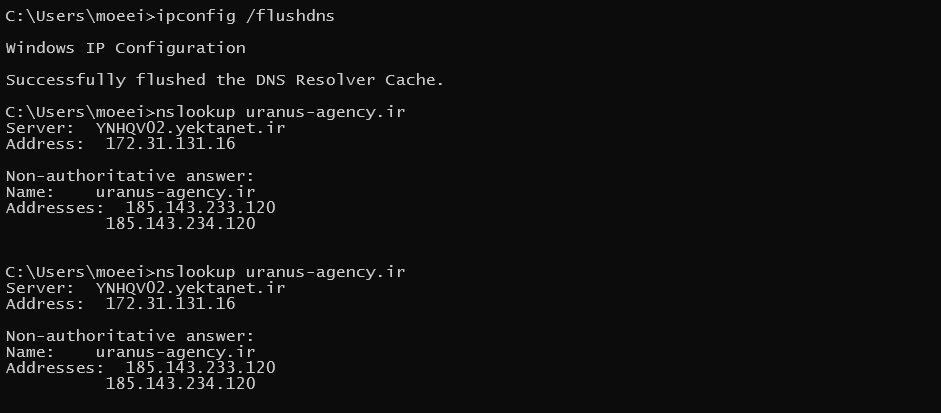
\includegraphics[width=0.8\textwidth]{screenshot007}
		
	}
}

همانطور که در تصویر مشخص است، از یک سرور DNS لوکال استفاده شده به نام 
\lr{YNHQV02.yektanet.ir}
که آدرس آیپی آن هم در تصویر موجود است. 

حال داخل wireshark فیلتر آیپی خودمان و فیلتر بسته‌های DNS را اعمال می‌کنیم تا بسته‌ها را مشاهده کنیم:

{
	\centering{
		
		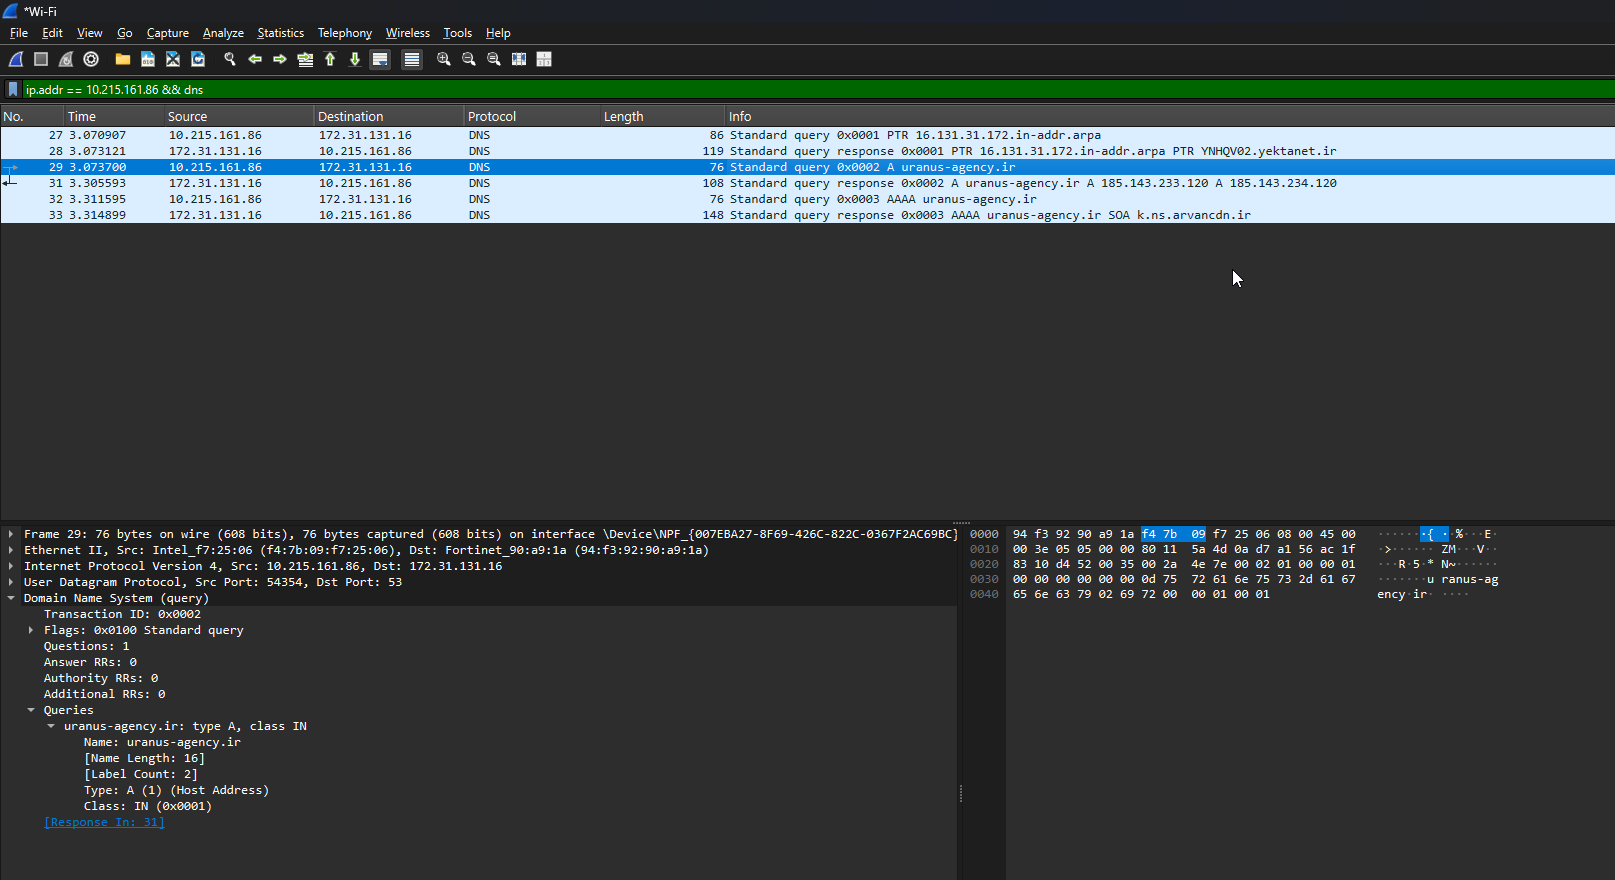
\includegraphics[width=0.8\textwidth]{screenshot008}
		
	}
}


\subsubsection*{سوال ۱.}

داخل بسته‌های فوق برای destination همان آدرس سرور DNS محلی که در تصاویر گذشته مشاهده کردیم نوشته شده است. پس بسته‌های کوئری استاندارد DNS‌ برای آن ارسال شده و پاسخ استاندارد هم از همان آدرس برای ما برمی‌گردد.

الته ما می‌توانیم سرور DNS را خودمان در دستور nslookup مشخص کنیم و آدرس آن را دستی وارد کنیم. اما اگر وارد نکنیم سلسه‌مراتب کوئری DNS اجرا می‌شود.

\pagebreak

\subsubsection*{سوال ۲.}


{
	\centering{
		
		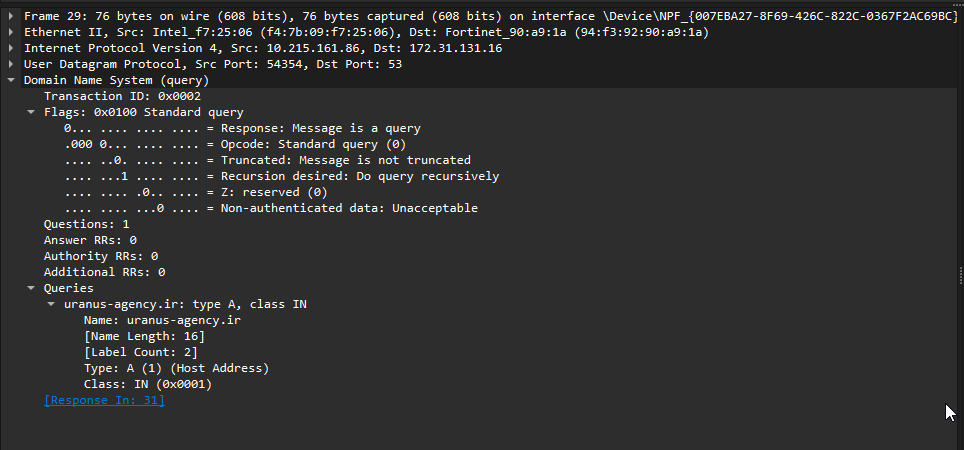
\includegraphics[width=1\textwidth]{screenshot009}
		
	}
}

یک نمونه بسته کوئری استاندارد به این صورت است. در اولین فلگ مشخص شده که این کوئری از نوع جواب است یا نه. که در این بسته مقدار 0 درج شده به این معنی که این بسته از نوع کوئری است. اما در پاسخ، مقدار این فلگ برابر ۱ شده است. همچنین داخل اطلاعات مربوط به کوئری نوشته شده که تایپ درخواست ما A است. پس رکورد A مربوط به دامنه‌ی درخواست داده شده را برای ما برمی‌گرداند.


{
	\centering{
		
		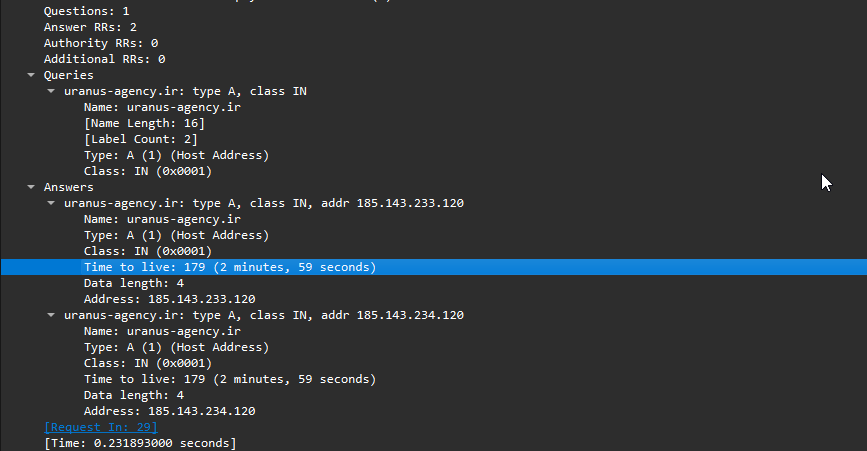
\includegraphics[width=1\textwidth]{screenshot010}
		
	}
}

داخل بسته پاسخ هم برای این درخواست ۲ جواب برگردانده شده است. پس این دامنه ۲ آیپی ادرس دارد که بین آن‌ها 
\lr{load balancing}
انجام می‌شود
. همچنین داخل جواب‌ها به ازای هر کدام از آیپی‌ها یک TTL برگردانده شده است که نشان می‌دهد ما می‌توانیم این مقدار را به مدت ۳ دقیقه در سرور DNS لوکال خود کش کنیم و پس از آن دوباره به سرور DNS اصلی کوئری ارسال کنیم.


{
	\centering{
		
		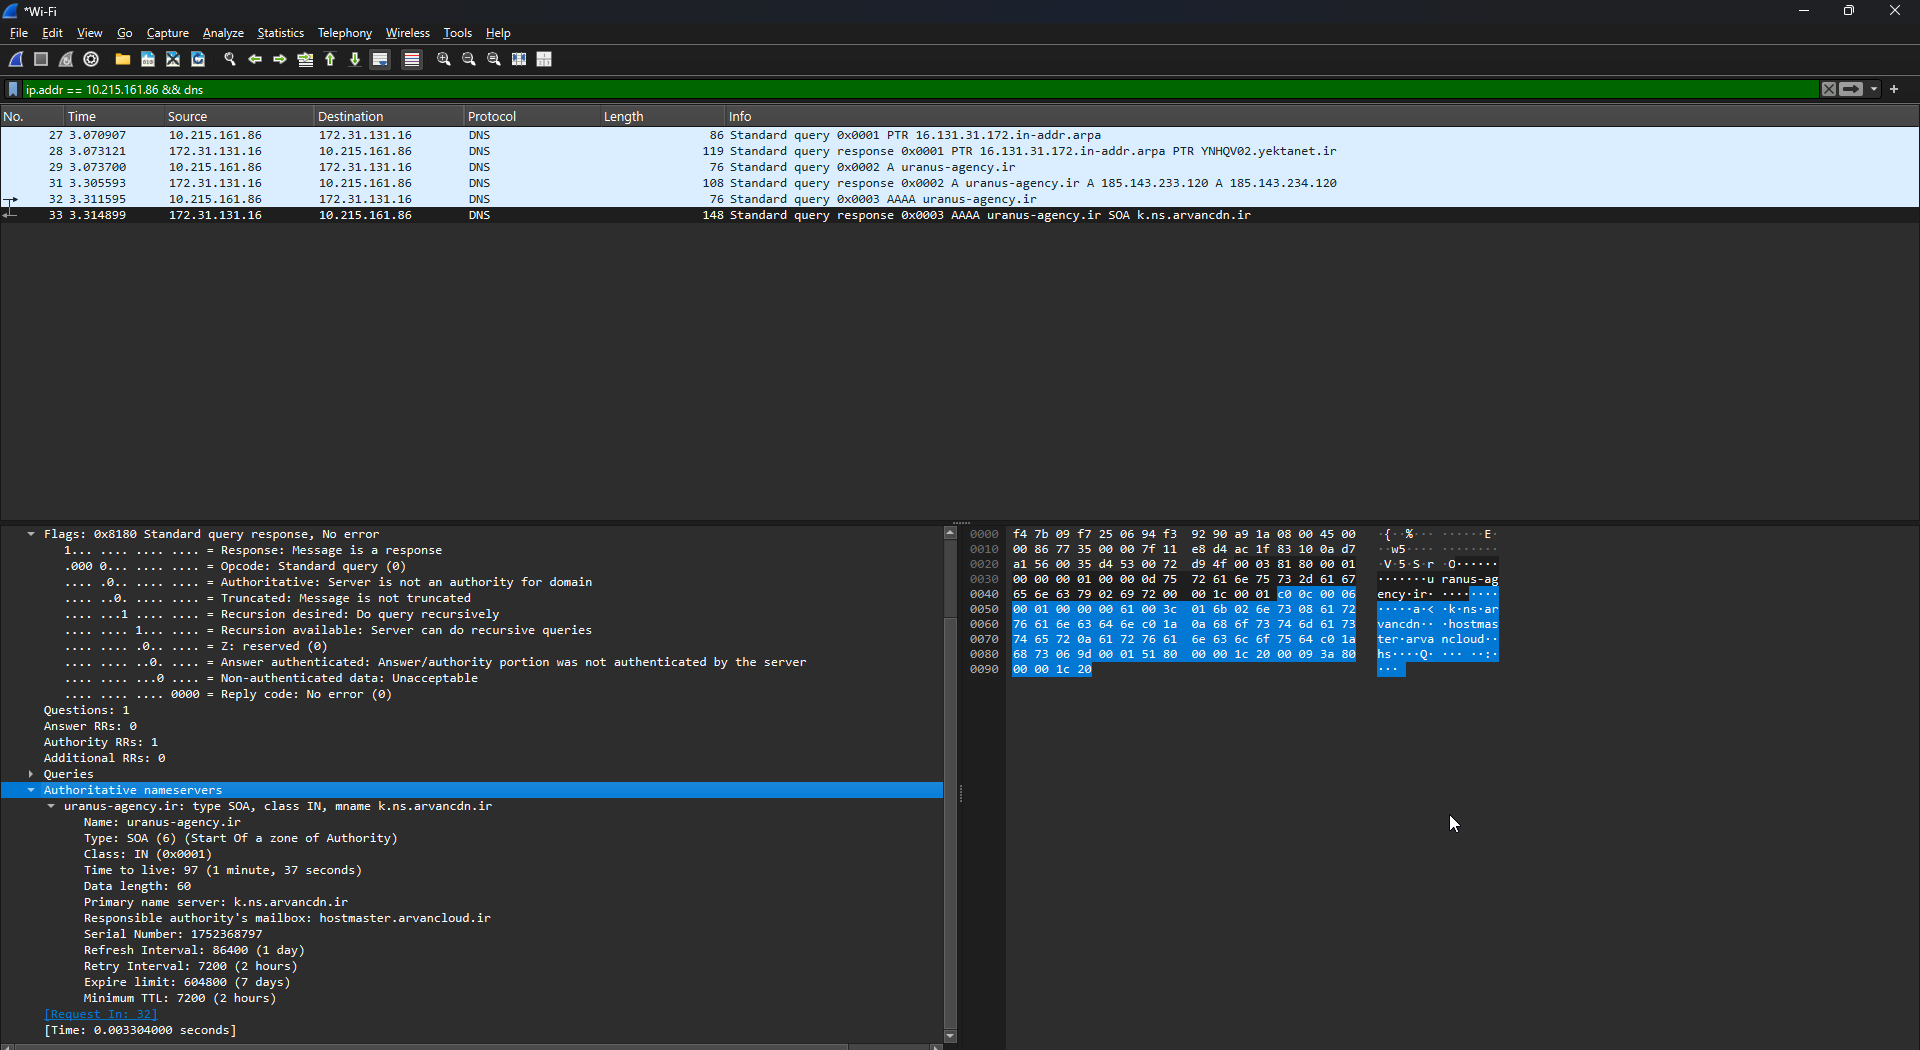
\includegraphics[width=1\textwidth]{screenshot011}
		
	}
}


پس از آن مشاهده می‌کنیم که یک کوئری از نوع AAAA هم برای به دست آوردن 
\lr{IPv6}
این دامنه ارسال شده است. اما چون برای این دامنه من آیپی ورژن ۶ تنظیم نکردم، در ریسپانس فقط اطلاعات 
\lr{Authoritative nameserver}
برگردانده شده است که مربوط به ابرآروان است.



همچنین باقی فلگ‌های موجود در هدر داخل بخش flags تصویر فوق قابل مشاهده است. جلوی هر کدام توضیحاتی نوشته شده که مشخص می‌کند هر کدام چه کاربردی دارند و مقدارشان در حال حاضر چند است.



